%%%%%%%%%%%%%%%%%%%%%%%%%%%%%%%%%%%%%%%%%
% Beamer Presentation
% LaTeX Template
% Version 1.0 (10/11/12)
%
% This template has been downloaded from:
% http://www.LaTeXTemplates.com
%
% License:
% CC BY-NC-SA 3.0 (http://creativecommons.org/licenses/by-nc-sa/3.0/)
%
%%%%%%%%%%%%%%%%%%%%%%%%%%%%%%%%%%%%%%%%%

%----------------------------------------------------------------------------------------
%	PACKAGES AND THEMES
%----------------------------------------------------------------------------------------

\documentclass[9pt]{beamer}

\mode<presentation> {

\usetheme{Berlin}

%\setbeamertemplate{footline} % To remove the footer line in all slides uncomment this line
\setbeamertemplate{footline}[page number] % To replace the footer line in all slides with a simple slide count uncomment this line

%\setbeamertemplate{navigation symbols}{} % To remove the navigation symbols from the bottom of all slides uncomment this line
}

\usepackage{graphicx} % Allows including images
\usepackage{booktabs} % Allows the use of \toprule, \midrule and \bottomrule in tables
\usepackage{verbatim} % Allows verbatim environments for code
\usepackage{textcomp} % Allows correct display of text in \texttt{}

\usepackage{listings}
\usepackage{xcolor}

\definecolor{darkgreen}{rgb}{0.0, 0.5, 0.0}  % Dark Green
\definecolor{darkpurple}{rgb}{0.5, 0.0, 0.5} % Dark Purple

\lstdefinestyle{mystyle}{
    language=C++,
    basicstyle=\ttfamily\footnotesize,
    keywordstyle=[1]\color{darkgreen}\bfseries, % C++ keywords
    keywordstyle=[2]\color{blue}, % alpaka related keywords
    identifierstyle=\color{black},
    commentstyle=\fontfamily{dvs}\selectfont\color{gray}, % Using Inconsolata for comments
    stringstyle=\color{red},
    numberstyle=\tiny\color{gray},
    numbers=left,
    numbersep=10pt,
    tabsize=2,
    breaklines=true,
    showstringspaces=false,
    escapeinside={(*@}{@*)},
    alsoletter={:}, % treat ':' as part of a keyword
    morekeywords={[1]auto, using, namespace, nullptr, static_cast, int, float, double, size_t, for, if, else, while, return}, % C++ keywords
    morekeywords={[2]alpaka, alpaka::PlatformCpu, alpaka::Vec, alpaka::Buf, alpaka::DevCpu, alpaka::Dev, alpaka::Platform, alpaka::KernelCfg, alpaka::WorkDivMembers, alpaka::AccGpuCudaRt, alpaka::AccGpuHipRt, alpaka::AccCpuThreads, alpaka::AccCpuOmp2Threads, alpaka::AccCpuOmp2Blocks, alpaka::AccCpuTbbBlocks, alpaka::AccCpuSerial, alpaka::AccGpuCudaRt} % alpaka keywords
}

\lstset{style=mystyle}

%----------------------------------------------------------------------------------------
%	TITLE PAGE
%----------------------------------------------------------------------------------------

\title[2D Heat Equation Simulation]{Heat Equation Simulation using Alpaka} % The short title appears at the bottom of every slide, the full title is only on the title page

\author{Alpaka Team} % Your name
\institute[HZDR] % Your institution as it will appear on the bottom of every slide, may be shorthand to save space
{
HZDR \\ % Your institution for the title page
\medskip
\textit{} % Your email address
}
\date{\today} % Date, can be changed to a custom date

\begin{document}

\begin{frame}
\titlepage % Print the title page as the first slide
\end{frame}

\begin{frame}
\frametitle{Overview} % Table of contents slide
\tableofcontents % Automatically prints the table of contents based on \section{} and \subsection{} commands
\end{frame}

%----------------------------------------------------------------------------------------
%	PRESENTATION SLIDES
%----------------------------------------------------------------------------------------

%------------------------------------------------
\section{Introduction} % Sections can be created to organize your presentation into discrete blocks
%------------------------------------------------
\begin{frame}
\vspace{-0.1\baselineskip} % This moves the text up by approximately two lines

\frametitle{The Heat Equation}
\scriptsize
\begin{itemize}
    \item \textbf{The heat equation models the Heat Diffusion over time in a given medium.}
    
    \[
    \frac{\partial u(x, y, t)}{\partial t} = \alpha \left( \frac{\partial^2 u(x, y, t)}{\partial x^2} + \frac{\partial^2 u(x, y, t)}{\partial y^2} \right)
    \]
\textbf{Difference approximations for Time and Spatial Derivatives:}
\begin{minipage}{0.45\textwidth}

     \[
\frac{\partial u(x, y, t)}{\partial t}\Bigg|_{t = t^n} \approx \frac{u_{i,j}^{n+1} - u_{i,j}^n}{\Delta t}
\]
\end{minipage}
\begin{minipage}{0.45\textwidth}

\[
\frac{\partial^2 u(x, y, t)}{\partial x^2}\Bigg|_{x = x_i, y = y_j} \approx \frac{u_{i+1,j}^n - 2u_{i,j}^n + u_{i-1,j}^n}{\Delta x^2}
\]
\end{minipage}
\item \textbf{Resulting difference equation:}
\[
u_{i,j}^{n+1} = u_{i,j}^n + \alpha \Delta t \left( \frac{u_{i+1,j}^n - 2u_{i,j}^n + u_{i-1,j}^n}{\Delta x^2} + \frac{u_{i,j+1}^n - 2u_{i,j}^n + u_{i,j-1}^n}{\Delta y^2} \right)
\]
\end{itemize}
\vspace{-0.3\baselineskip}
\begin{figure}
    \centering
    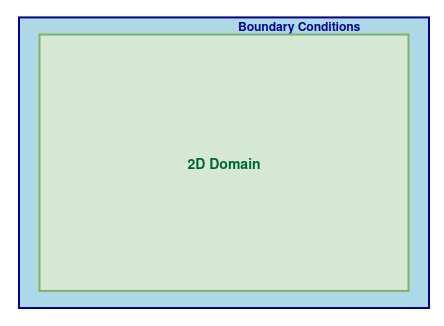
\includegraphics[width=0.45\linewidth,height=0.35\linewidth]{Screenshot from 2024-08-30 14-04-56.png}
\end{figure}
\end{frame}
%------------------------------------------------
\section{Domain and Stencil}
%------------------------------------------------
% All domain etc
\begin{frame}
\frametitle{Parallel Heat Equation Solution}
\vspace{-0.5\baselineskip}
\scriptsize
    \begin{itemize}
        \item \textbf{Data Parallelism:} Each point on the grid can be updated independently based on its neighbors, enabling parallel computation.
        \item \textbf{Stencil Operations:} Stencil is a core computational pattern in PDE solvers. Updates a grid point in time using its immediate neighbors (left, right, up, down) according to the difference equation. A 5-point stencil is needed.
    \end{itemize}    
    %first image without blocks
    \vspace{-0.5\baselineskip}
    \begin{figure}
        \centering
        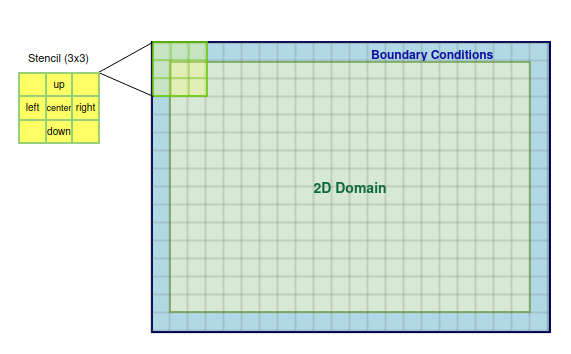
\includegraphics[width=0.6\linewidth]{Screenshot from 2024-08-30 14-18-30.png}
        \label{fig:enter-label}
    \end{figure}
    \begin{itemize}
        \item \textbf{Halo Region for BC:} A layer of grid cells surrounding the problem domain for Boundary Conditions.
        \begin{itemize}
            \item Facilitates stencil operations at the boundaries of subdomains.
        \end{itemize}
    \end{itemize}
\end{frame}

\begin{frame}
\frametitle{Calculation of $u_{i,j}^{n+1}$ from $u_{i,j}^{n}$}
\vspace{-0.9\baselineskip}
    \begin{itemize}
        \item Each kernel execution by alpaka calculates $u_{i,j}^{n+1}$ using $u_{i,j}^{n}$
        \item Each heat point is separately calculated by a thread using frobenious inner product
        \item Calculation of $u_{0,0}^{n+1}$ by a single thread
    \end{itemize}
    \begin{figure}
        \centering
        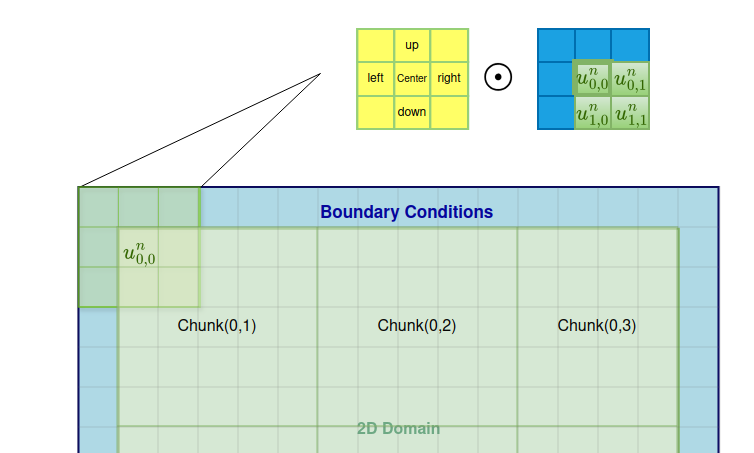
\includegraphics[width=0.85\linewidth]{Screenshot from 2024-09-02 13-42-49.png}
        \caption{First thread calculates $u_{0,0}^{n+1}$ using frobenious inner product of 3x3 matrices}
        \label{fig:enter-label}
    \end{figure}
\end{frame}

\begin{frame}
\vspace{-0.9\baselineskip}
    \begin{itemize}
        \item Second thread calculates $u_{0,1}^{n+1}$  
    \end{itemize}
    \begin{figure}
        \centering
        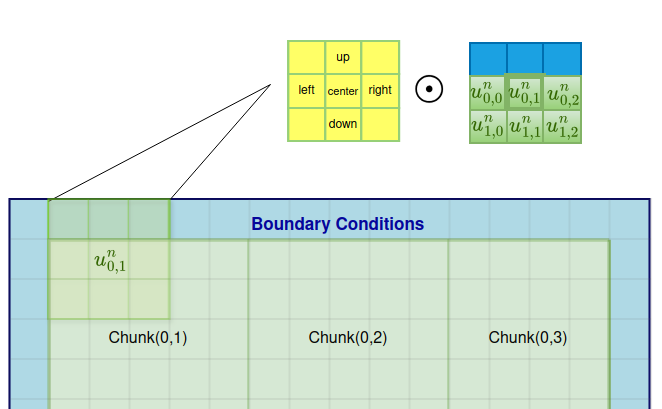
\includegraphics[width=0.85\linewidth]{Screenshot from 2024-09-02 13-53-13.png}
        \caption{Second thread calculates $u_{0,1}^{n+1}$ using }
        \label{fig:enter-label}
    \end{figure}
\end{frame}

%------------------------------------------------
\section{Parallelization}
%------------------------------------------------

\begin{frame}
\frametitle{Chunks in Parallel Grid Computations}
\begin{itemize}
%    \item \textbf{Halo Region For Shared:} A layer of block cells surrounding the main computational domain.
 
    \item \textbf{Chunk:} Subdomains needed for block level parallelisation
    \item \textbf{Halo Region around chunk:} A layer of grid cells surrounding the subdomains. In order to use the heat value beside the current chunk
    \item \textbf{Halo Size:} Typically 1 for a 5-point stencil.
\end{itemize}

\begin{figure}
    \centering
    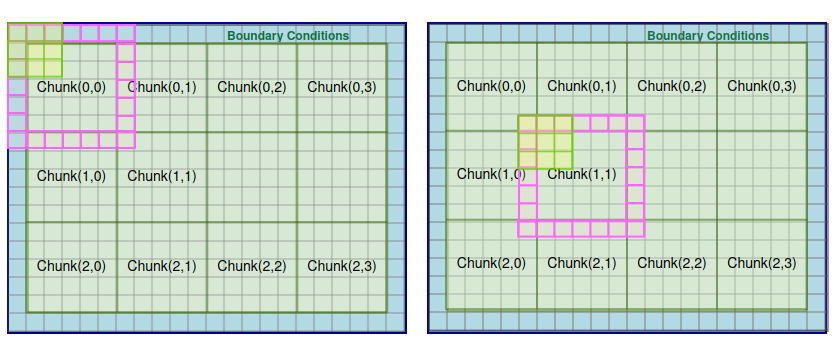
\includegraphics[width=0.8\linewidth]{Screenshot from 2024-08-30 19-03-50.png}
   % \caption{Chunks deviding the domaing and the defined halo regions}
    \label{fig:enter-label}
\end{figure}
\end{frame}

\begin{frame}
\frametitle{Chunk Definition (in detail?)}
\begin{figure}
    \centering
    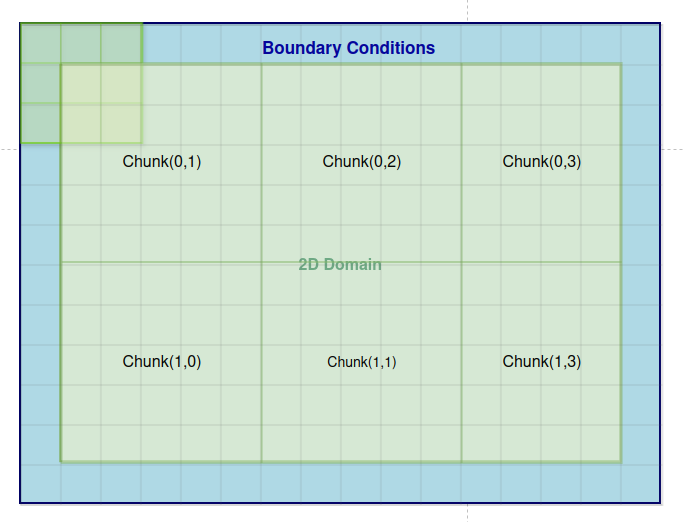
\includegraphics[width=0.85\linewidth]{Screenshot from 2024-09-02 14-11-22.png}
    \caption{Heat values correponding to each chunk is updated by a block}
    \label{fig:enter-label}
\end{figure}
\end{frame}

%------------------------------------------------
\section{Simulation Setup using Alpaka}
%------------------------------------------------
% mention dont provide code or detailed info
\begin{frame}[fragile]
\frametitle{Accelerator, Device and Host}
\textbf{Define number of dim and index type}
\begin{lstlisting}
using Dim = alpaka::DimInt<2u>; // Number of dim: 2 as a type
using Idx = std::size_t; // Index type of the threads and buffers
\end{lstlisting}

\textbf{Define the accelerator}
\begin{lstlisting}
// AccGpuCudaRt, AccGpuHipRt, AccCpuThreads, AccCpuSerial,
// AccCpuOmp2Threads, AccCpuOmp2Blocks, AccCpuTbbBlocks 
using Acc = alpaka::AccGpuCudaRt<Dim, Idx>;
using DevAcc = alpaka::Dev<Acc>;
\end{lstlisting}
\textbf{Select a device from platform of Acc}
\begin{lstlisting}
auto const platform = alpaka::Platform<Acc>{};
auto const devAcc = alpaka::getDevByIdx(platform, 0);
\end{lstlisting}
\textbf{Select a host and hosttype to allocate memory for data}
\begin{lstlisting}
// Get the host device for allocating memory on the host.
auto const platformHost = alpaka::PlatformCpu{};
auto const devHost = alpaka::getDevByIdx(platformHost, 0);
// Host device type is needed, still not known
using DevHost = alpaka::DevCpu;
\end{lstlisting}
\end{frame}

 \begin{frame}[fragile]
\frametitle{Allocate memory at Host and at Device}

\begin{lstlisting}

// Allocate host memory buffers
using BufHost = alpaka::Buf<DevHost, DataType, Dim, Idx>;
BufHost bufHostA(alpaka::allocBuf<DataType, Idx>(devHost, extent));
 
// Fill the host buffers
for (Idx i(0); i < numElements; ++i) {
    bufHostA[i] = randomA;
}

// Allocate buffer on the accelerator
using BufAcc = alpaka::Buf<DevAcc, DataType, Dim, Idx>;
BufAcc bufAccA(alpaka::allocBuf<DataType, Idx>(devAcc, extent));
\end{lstlisting}
\end{frame}


 \begin{frame}[fragile]
\frametitle{Need a queue to copy the data to the device}

\begin{lstlisting}
    using Acc = alpaka::AccCpuSerial<Dim, Idx>;
    auto const platformAcc = alpaka::Platform<Acc>{};
    auto const devAcc = alpaka::getDevByIdx(platformAcc, 0);
    // A queue is needed for all acc related operations
    alpaka::Queue<Acc, alpaka::Blocking> queue(devAcc);

    // Define the 2D extents (dimensions)
    Vec const extentA(static_cast<Idx>(M), static_cast<Idx>(K));

    // Allocate host memory, the memory size is determined by extent
    auto bufHostA = alpaka::allocBuf<DataType, Idx>(devHost, extentA);

    // Allocate device memory
    auto bufDevA = alpaka::allocBuf<DataType, Idx>(devAcc, extentA);

    // Copy data to device, use host buffer and device buffer
    // Queue must be an accelerator queue
    alpaka::memcpy(queue, bufDevA, bufHostA);

\end{lstlisting}
\end{frame}

\begin{frame}[fragile]
\scriptsize
\frametitle{Passing multi dimentional data to the kernel}
Multi-dimentional memory allocated in memory uses aligned rows.

Hence, if a pointer of a 2D buffer is passed to the kernel as a pointer; 2 additional values \textbf{pitch} and item \textbf{data-size} should also be passed.


\begin{columns} % Create columns
    \begin{column}{0.55\textwidth} % Adjust the width to your preference
        % Left column with text
    
        \textbullet \hspace{0.5em} \textbf{Pass 3 variables to kernel: pointer, pitch, and datasize}
            
        \lstset{basicstyle=\ttfamily\tiny} 
        \begin{lstlisting}
    template<typename TAcc, typename TDim, typename TIdx>
    ALPAKA_FN_ACC auto operator()(
        TAcc const& acc,
        double const* const uCurrBuf,
        double* const uNextBuf,
        alpaka::Vec<TDim, TIdx> const pitchCurr,
        alpaka::Vec<TDim, TIdx> const pitchNext,
        ...) const -> void
        \end{lstlisting}
    \end{column}

    \begin{column}{0.48\textwidth} % Adjust the width to your preference
        % Right column with the image
        \hspace{-0.2\baselineskip}
        \centering
 
     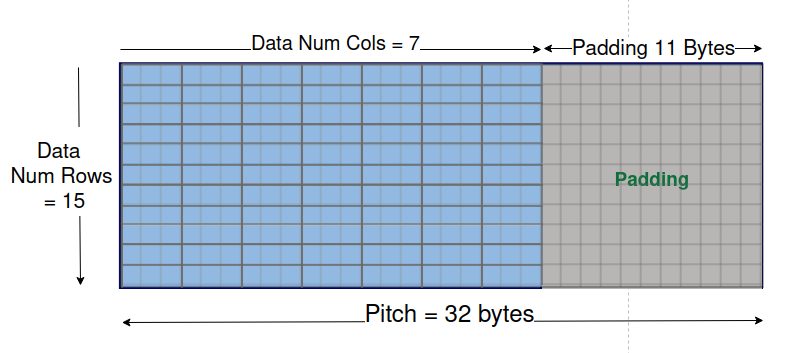
\includegraphics[width=1\linewidth]{Screenshot from 2024-09-04 17-16-43.png}
     \caption{2D Buffer with size 15x7 in memory}
     \label{fig:enter-label}
 
        % Replace 'example-image.png' with your image filename
    \end{column}
\end{columns}
\textbullet \hspace{0.5em} \textbf{Simple Alternative: Pass an alpaka::mdspan object}
\lstset{basicstyle=\ttfamily\tiny} 
\begin{lstlisting}
    template<typename TAcc, typename TDim, typename TIdx, typename TMdSpan>
    ALPAKA_FN_ACC auto operator()(
        TAcc const& acc,
        TMdSpan uCurrBuf,
        TMdSpan uNextBuf
        ...) const -> void
\end{lstlisting}

\end{frame}

\section{WorkDiv: How to parallelize? }
%------------------------------------------------
% mention dont provide code or detailed info

\begin{frame}[fragile]
\frametitle{WorkDiv-I: Setting workdiv fields directly}

\begin{lstlisting}
auto blocksPerGrid = alpaka::Vec<Dim, Idx>{M/8, N/128};
auto threadsPerBlock = alpaka::Vec<Dim, Idx>{8, 128};
auto elementsPerThread = alpaka::Vec<Dim, Idx>{1u, 1u};
using WorkDiv = alpaka::WorkDivMembers<Dim, Idx>;
auto workDiv = WorkDiv{blocksPerGrid, threadsPerBlock, elementsPerThread};
\end{lstlisting}

\begin{figure}
    \centering
    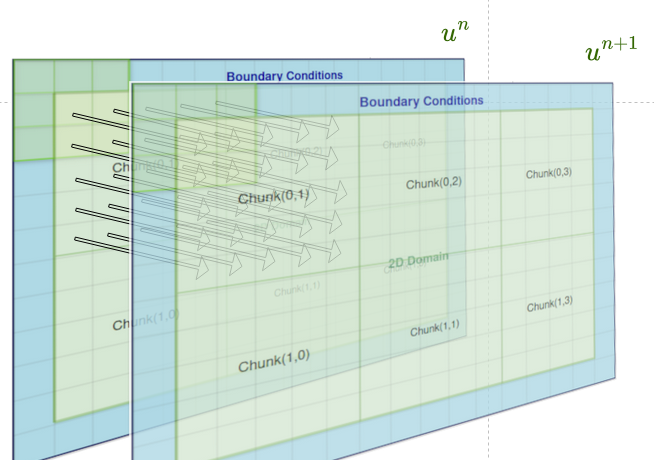
\includegraphics[width=0.75\linewidth]{Screenshot from 2024-09-04 13-55-10.png}
    \caption{Enter Caption}
    \label{fig:enter-label}
\end{figure}
\end{frame}


\begin{frame}[fragile]
\frametitle{WorkDiv-II: Let Alpaka calculate for you}

\begin{lstlisting}
using Acc = alpaka::AccCpuSerial<Dim, Idx>;
auto const devAcc = alpaka::getDevByIdx(platformAcc, 0);

// Define the 2D extents as {Width, Height} of matrix
alpaka::Vec<Dim, Idx> const extentAsThreadsPerGrid(M, N);
auto elementsPerThread = alpaka::Vec<Dim, Idx>{1u, 1u};
MatrixMulKernel kernel;

// Let alpaka calculate good block and grid sizes given our full problem extent
alpaka::KernelCfg<Acc> const kernelCfg = {extentAsThreadsPerGrid, elementsPerThread};
auto const workDiv = alpaka::getValidWorkDiv<Acc>(kernelCfg, devAcc, kernel, // kernel params here
);
\end{lstlisting}
\end{frame}


%------------------------------------------------
\section{Execution}
%------------------------------------------------

\begin{frame}
\frametitle{Main Simulation Loop: Leveraging Parallelism}
\begin{itemize}
    \item \textbf{Initialization:}
    \begin{itemize}
        \item Define the "host device" and "accelerator device". The "Host" and "Device" in short.
        \item Set initial conditions and boundary conditions.
        \item Allocate data buffers to host and device.
        \item Copy data from host to device buffer to pass to the kernel.
        \item Define parallelisation strategy (chunk size, block size, etc.).
    \end{itemize}
    \item \textbf{Simulation Loop:}
    \begin{itemize}
        \item \textbf{Step 1:} Execute \texttt{StencilKernel} to compute next values.
        \item \textbf{Step 2:} Apply boundary conditions using \texttt{BoundaryKernel}.
        \item \textbf{Step 3:} Swap buffers for the next iteration so that calculated  $u_{i,j}^{n+1}$ becomes the $u_{i,j}^{n}$ for the next step.
    \end{itemize}
    \item \textbf{Parallel Efficiency:}
    \begin{itemize}
        \item Subdomains are processed in parallel, with halos ensuring data consistency and correct boundary conditions.
        \item Optimization: Shared memory optimizes memory access within each block.
    \end{itemize}
    \item \textbf{Validation}
\end{itemize}
\end{frame}

\begin{frame}
\frametitle{Executing the Kernel}
\begin{itemize}
    \item \textbf{Execution Flow:}
    \begin{itemize}
        \item Each kernel is executed on the selected accelerator (e.g., CPU, GPU).
        \item Halo regions and shared memory are leveraged for optimal parallel performance.
    \end{itemize}
    \item \textbf{Kernel Execution:} \\
    \texttt{alpaka::exec<Acc>(} \\
    \texttt{queue1,} \\
    \texttt{workDiv\_manual,} \\
    \texttt{stencilKernel,} \\
    \texttt{uCurrBufAcc.data(),} \\
    \texttt{uNextBufAcc.data(),} \\
    \texttt{chunkSize,} \\
    \texttt{dx, dy, dt);} \\
    \item \textbf{Run Example:} Execute for all enabled accelerators (e.g., CUDA, HIP, OpenMP).
\end{itemize}
\end{frame}

%------------------------------------------------

%------------------------------------------------
% mention dont provide code or detailed info
\begin{frame}
\frametitle{Applying Boundary Conditions in Parallel}
\begin{itemize}
    \item \textbf{Boundary Kernel:} Ensures correct values at the boundaries of the grid.
    \item \textbf{Challenges in Parallel Computing:}
    \begin{itemize}
        \item Boundary points might need special handling, particularly when subdomains are processed independently.
        \item Halo regions play a crucial role here.
    \end{itemize}
    \item \textbf{Code Snippet:} \\
    \texttt{if (gridBlockIdx[0] == 0) \{} \\
    \texttt{applyBoundary(globalIdx, chunkSize[1], true);} \\
    \texttt{\}}
\end{itemize}
\end{frame}

%------------------------------------------------
\section{Optimization}
%------------------------------------------------
% Will go down because this is optimization: opt is shared memory, 2 queues
% 
\begin{frame}
\frametitle{Efficient Stencil Computation with Shared Memory}
\begin{itemize}
    \item \textbf{Shared Memory:}
    \begin{itemize}
        \item A fast, limited-size memory accessible by all threads within a block.
        \item Used to store grid points locally, reducing the need to access slower global memory.
    \end{itemize}
    \item \textbf{Benefits:}
    \begin{itemize}
        \item Reduces memory latency by storing the working set of data (halo + core) in shared memory.
        \item Enables efficient data reuse across threads in the same block.
    \end{itemize}
    \item \textbf{Example:} \\
    \texttt{auto\& sdata = alpaka::declareSharedVar<double[T\_SharedMemSize1D], \_\_COUNTER\_\_>(acc);}
    \item \textbf{Synchronization ...I/O:} 
    \begin{itemize}
        \item Threads in a block must synchronize to ensure all data is loaded into shared memory before computation begins.
    \end{itemize}
\end{itemize}
\end{frame}

%------------------------------------------------
% mention dont provide code or detailed info
\begin{frame}
\frametitle{Using multiple queues}

\end{frame}
%------------------------------------------------

\begin{frame}
\frametitle{Results and Performance in Parallel Execution}
\begin{itemize}
    \item \textbf{Validation:} 
    \begin{itemize}
        \item Accuracy of results compared to the analytical solution.
        \item Performance considerations: Speedup achieved by parallelizing the computation.
    \end{itemize}
    \item \textbf{Output:}
    \begin{itemize}
        \item Print whether the results are correct.
        \item Report on the maximum error.
        \item Discuss any performance metrics (e.g., execution time).
    \end{itemize}
    \item \textbf{Visual Output (Optional):}
    \begin{itemize}
        \item Periodic snapshots of the temperature distribution.
    \end{itemize}
\end{itemize}
\end{frame}

%------------------------------------------------
\section{Conclusion}
%------------------------------------------------

\begin{frame}
\frametitle{Conclusion: Parallel Techniques for Efficient Simulation}
\begin{itemize}
    \item \textbf{Key Takeaways:}
    \begin{itemize}
        \item Efficient use of shared memory significantly boosts performance in parallel computations.
        \item Halo regions are crucial for managing data dependencies in stencil operations.
        \item The combination of Alpaka’s abstraction and careful memory management enables scalable and portable parallel solutions.
    \end{itemize}
\end{itemize}
\end{frame}

%------------------------------------------------

\begin{frame}
\Huge{\centerline{Questions?}}
\end{frame}

%----------------------------------------------------------------------------------------

\end{document}
